\documentclass[11pt]{article}
%\usepackage[paperwidth=8.5in, paperheight=11in]{geometry}
\usepackage[a5paper, landscape]{geometry}
\usepackage{tikz}

\usepackage{../tjimo}
%\usepackage{graphicx}
%\usepackage[pdftex]{graphicx}

\newcommand{\sevenpoints}{Time limit: 40 minutes.}
\newcommand{\righthead}{\fdbox{Round}{Guts Solutions}}

%\def\newpage{}
%\begin{comment}
\def\answer{\comment}
\def\solution{\comment}
\renewcommand{\righthead}{\fdbox{Round}{Guts}}
\setlength{\headheight}{11em}
\setlength{\footskip}{0em}
\rfoot{\emph{\sevenpoints}\vspace{5em}}
%\end{comment}

\DeclareMathOperator{\lcm}{lcm}

\begin{document}

\section*{Set 1}
\begin{problem}
What is $1 + 2 + 3 + 4 + \dots + 100$?
\end{problem}

\begin{answer}
5050
\end{answer}

\begin{solution}
Note that $100+1=99+2=98+3=\cdots=51+50=101$. Since there are $\frac{100}{2}=50$ of these pairs, we see that the sum is $50(101)=\boxed{5050}$.
\end{solution}


\begin{problem}
Miranda is picking out skirts and crop tops to wear. If she has 5 skirts and 7 crop tops, how many outfits can she make?
\end{problem}

\begin{answer}
35
\end{answer}

\begin{solution}
Note that for every skirt, Miranda can wear any of the seven crop tops. This gives us a total of $5 \cdot 7 = \boxed{35}$ outfits. 
\end{solution}


\begin{problem}
What is the least common multiple of 6 and 4?
\end{problem}

\begin{answer}
12
\end{answer}

\begin{solution}
Since $6=2\cdot 3$ and $4=2^2$, the LCM is $2^2 \cdot 3=\boxed{12}$.
\end{solution}


\begin{problem}
How many multiples of $7$ are between $100$ and $200$?
\end{problem}

\begin{answer}
14
\end{answer}

\begin{solution}
The multiples of $7$ between $100$ and $200$ are: \[ 15 \cdot 7, 16 \cdot 7, \cdots, 27 \cdot 7, 28 \cdot 7 \]
There are $28 - 15 + 1 = \boxed{14}$ such multiples of $7$.
\end{solution}


\newpage
\section*{Set 2}
\begin{problem}
Gibbons drinks $\frac{1}{3}$ of the water in a bottle, and Ogden drinks $\frac{1}{4}$ of the remaining water. If there are 8 milliliters of water left, how much water (in milliliters) was there to begin with?
\end{problem}

\begin{answer}
16
\end{answer}

\begin{solution}
Gibbons drinks $\frac{1}{3}$ of the water, and Ogden drinks $\frac{2}{3} \cdot \frac{1}{4} = \frac{1}{6}$ of the water, leaving $1-\frac{1}{3} - \frac{1}{6} = \frac{1}{2}$ of the water remaining. Since $\frac{1}{2}$ of the water is 8 mL, there must have been $\boxed{16}$ mL of water to start with.
\end{solution}


\begin{problem}
I am drawing marbles out of a bag. If the bag contains 3 red marbles and 5 blue marbles, then what is the probability that the second marble I draw is red?
\end{problem}

\begin{answer}
$\frac{3}{8}$
\end{answer}

\begin{solution}
Note that the probability that the second marble is red is equal to the probability that the first marble is red, because we can always just swap the order we selected the first two marbles. Thus, the answer is $\frac{3}{3+5} = \boxed{\frac{3}{8}}$.
\end{solution}


\begin{problem}
How many positive integer factors does 27 have? 
\end{problem}

\begin{answer}
4
\end{answer}

\begin{solution}
Since $27 = 3^3$, the only factors are 1, 3, 9, and 27, giving us a total of $\boxed{4}$ factors.
\end{solution}


\begin{problem}
In the diagram below, if the radius of the larger circle is $6$, and all the smaller circles are the same size, then what is the side length of the hexagon?
    \begin{center}
        \begin{tikzpicture}[thick, scale=0.6]
            \draw (0, 0) circle (3cm);
            \draw (0, 0) circle (1cm);
            \draw (2, 0) circle (1cm);
            \draw (-2, 0) circle (1cm);
            \draw (1, 1.73205080757) circle (1cm);
            \draw (1, -1.73205080757) circle (1cm);
            \draw (-1, 1.73205080757) circle (1cm);
            \draw (-1, -1.73205080757) circle (1cm);
            \draw (2, 0) -- (1, 1.73205080757) -- (-1, 1.73205080757) -- (-2, 0) -- (-1, -1.73205080757) -- (1, -1.73205080757) -- cycle;
        \end{tikzpicture}
    \end{center}
\end{problem}

\begin{answer}
4
\end{answer}

\begin{solution}
Consider the following diagram. 
    \begin{center}
        \begin{tikzpicture}[thick, scale=0.6]
            \draw (0, 0) circle (3cm);
            \draw (0, 0) circle (1cm);
            \draw (2, 0) circle (1cm);
            \draw (-2, 0) circle (1cm);
            \draw (1, 1.73205080757) circle (1cm);
            \draw (1, -1.73205080757) circle (1cm);
            \draw (-1, 1.73205080757) circle (1cm);
            \draw (-1, -1.73205080757) circle (1cm);
            \draw (2, 0) -- (1, 1.73205080757) -- (-1, 1.73205080757) -- (-2, 0) -- (-1, -1.73205080757) -- (1, -1.73205080757) -- cycle;
            \draw[color = red] (0, 0) -- (2, 0);
            \draw[color = blue] (0, 0) -- (1.5, 2.59807621);
        \end{tikzpicture}
    \end{center}

Note that if we draw in the horizontal segment across two radii, it is equal to the side-length of the hexagon. 
Thus, the length of the hexagon is equal to two times the radius of a smaller circle. Also note that the radius of a smaller circle is equal to 
$\frac{1}{3}$ of the radius of the larger circle. Thus, the side length of the hexagon is equal to 
$2 \cdot \frac{1}{3}=\frac{2}{3}$ of the larger radius, or $\frac{2}{3} \cdot 6 = \boxed{4}$.
\end{solution}


\newpage
\section*{Set 3}
\begin{problem}
If $A+B=4$, $C+D=8$, and $A+C=7$, what is $B+D$?
\end{problem}

\begin{answer}
5
\end{answer}

\begin{solution}
Adding the first two equations yields $A+B+C+D=12$. Subtracting $A+C=7$ gives us $B+D=\boxed{5}$.
\end{solution}


\begin{problem}
There is a 40\% chance of rain on Saturday. If it rains on Saturday, there is a 60\% chance of rain on Sunday. Otherwise, there is a 30\% chance of rain on Sunday. What is the probability it rains on Sunday?
\end{problem}

\begin{answer}
0.42
\end{answer}

\begin{solution}
If it rains on Saturday, there is a probability of $0.4 \cdot 0.6 =  0.24$ that it will rain on Sunday. If it doesn't rain on Saturday, there is a probability of $0.6 \cdot 0.3 = 0.18$ that it will rain on Sunday. Adding these up yields our desired answer of $\boxed{0.42}$.
\end{solution}


\begin{problem}
The least common multiple of the first ten positive integers is $2520$. What is the least common multiple of the first eleven positive integers?
\end{problem}

\begin{answer}
27720
\end{answer}

\begin{solution}
We want the smallest positive integer divisible by the first $11$ positive integers. We know that every multiple of $2520$ is divisible by the first $10$ positive integers, so our desired least common multiple must be $2520 \cdot 11 = \boxed{27720}$.
\end{solution}


\begin{problem}
Point $C$ is the center of the rectangle shown below. If the area of the whole rectangle is $128$, find the area of the shaded region.
\begin{center}
\begin{asy}
size(100);
draw((0,0)--(5,0)--(5,3)--(0,3)--(0,0));
draw((0,1.5)--(2.5, 1.5));
draw((2.5,1.5)--(5, 0));
dot((2.5, 1.5));
label("C", (2.5, 1.5), NE);
fill((0,0)--(0,1.5)--(2.5,1.5)--(5, 0)--(0,0)--cycle,gray);
\end{asy}
\end{center}
\end{problem}
\begin{answer}
$20$
\end{answer}
\begin{solution}
Extend the lines in the diagram as such: 
\begin{center}
\begin{asy}
size(100);
draw((0,0)--(5,0)--(5,3)--(0,3)--(0,0));
draw((0,1.5)--(5, 1.5));
draw((2.5,0)--(2.5,3));
draw((0,3)--(5, 0));
draw((0,0)--(5, 3));
dot((2.5, 1.5));
label("C", (2.5, 1.5), NE);
fill((0,0)--(0,1.5)--(2.5,1.5)--(5, 0)--(0,0)--cycle,gray);
\end{asy}
\end{center}
We divided the rectangle into eight congruent triangles, three of which are shaded. Thus $\dfrac{3}{8}$ of the total area is shaded, so our answer is $128 \cdot \dfrac{3}{8} = \boxed{48}.$
\end{solution}


\newpage
\section*{Set 4}
\begin{problem}
Let the function $f(x)$ be defined as $f(x) = 3x^2 + 2x + 3^{800}$. Find $f(3) - f(2)$.
\end{problem}

\begin{answer}
$17$
\end{answer}

\begin{solution}
Notice $f(3) - f(2) = 3(3)^2 + 2(3) + 3^{800} - (3(2)^2 + 2(2) + 3^{800}) = 27 + 6 - 12 - 4 = \boxed{17}$.
\end{solution}


\begin{problem}
Suppose $a$ and $b$ are positive integers such that $ab = 1296$ and neither $a$ nor $b$ is divisible by $6$. Find $a+b$.
\end{problem}

\begin{answer}
97
\end{answer}

\begin{solution}
Notice $ab = 1296 = 6^4 = 3^4 \cdot 2^4$. Since neither $a$ nor $b$ is divisible by $6$, neither $a$ nor $b$ can have both a factor of $3$ and a factor of $2$. Thus, one of $a,b$ must be $3^4$ and the other must be $2^4$, so our answer is $a+b = 3^4 + 2^4 = 81 + 16 = \boxed{97}$.
\end{solution}


\begin{problem}
Let $a$ be a solution to the equation $x^2 + 7x - 16 = 0$. Find the product of $a$ and $a+7$.
\end{problem}

\begin{answer}
$\boxed{16}$.
\end{answer}

\begin{solution}
We know that $a^2 + 7a - 16 = 0$, so $a(a+7) = a^2 + 7a = \boxed{16}$.
\end{solution}


\begin{problem}
How many ways can I seat Josh, Akshaj, Jeffery, Katherine, Michael, and Wendy at a circular table, where all seats are numbered
and distinguishable, so that Wendy and Katherine are sitting next to each other?
\end{problem}

\begin{answer}
288
\end{answer}

\begin{solution}
Let us fix Wendy and Katherine in two adjacent seats. Then, there are $4!=24$ ways to arrange the other 4 people. However, there are two ways for Wendy and Katherine to occupy a pair of adjacent seats (Wendy and Katherine can switch seats), and there are six such pairs Wendy and Katherine could have selected, so there are a total of $24 \cdot 2 \cdot 6 = \boxed{288}$ ways.
\end{solution}


\newpage
\section*{Set 5}
\begin{problem}
For an art project, Katherine is building a model of TJ. If the real auditorium is 30 feet wide, and the auditorium in Katherine's model is
2 inches wide, how long in inches should the model gym be if the real gym is 75 feet long?
\end{problem}

\begin{answer}
$5$
\end{answer}

\begin{solution}
Using proportions, we see that $\frac{2}{30} = \frac{x}{75}$, where $x$ is the length of the gym of the model in inches. Solving for $x$ gives $x=\boxed{5}$ inches.
\end{solution}


\begin{problem}
A 5-year-old, a 6-year-old, a 7-year-old, and an 8-year-old come to Akshaj's house for trick-or-treating during Halloween. Akshaj has $7$ identical pieces of candy to give out. How many ways can Akshaj distribute his $7$ pieces of candy among the four children, assuming each child must receive at least one piece of candy?
\end{problem}

\begin{answer}
20
\end{answer}

\begin{solution}
Akshaj can start by handing out one piece of candy to each child. Then he has three pieces left over to hand out. He can either \begin{enumerate} \item give all three pieces to the same child, \item give two pieces to one child and one to another, \item or give one piece to each of three children and leave one out. \end{enumerate}
In the first case, there are $4$ ways to choose which child to give the three pieces to. In the second case, there are $4 \cdot 3$ ways to choose the children to give two and one pieces of candy to. In the last case, there are $4$ ways to choose which child to leave out. Our final answer is $4 + 4 \cdot 3 + 4 = \boxed{20}$.
\end{solution}


\begin{problem}
What is the probability that if I flip a coin 5 times in a row, I get heads at least 3 times?
\end{problem}

\begin{answer}
$\frac{1}{2}$
\end{answer}

\begin{solution}
Notice that I get heads at least $5$ times if and only if I get more heads than tails. 
Thus, we need only find the probability that we flip more heads than tails. By symmetry, this is equal to the probability of flipping more 
tails than heads. Since $5$ is odd, all possible sequences of flips must result in either having more heads than tails or more 
tails than heads, so our desired probability is exactly $\boxed{\dfrac{1}{2}}$.
\end{solution}


\begin{problem}
Gideon is facing trial, but he only has 10 dollars. If Wainwright offers lawyers for 3 dollars and investigators for 2 dollars each, 
how many combinations of lawyers and investigators can Gideon hire, assuming that he needs to hire at least one lawyer and he does not 
need to spend all 10 dollars? (For example, Gideon can hire one lawyer and no investigators.)
\end{problem}

\begin{answer}
8
\end{answer}

\begin{solution}
Since Gideon needs to hire a lawyer, the problem is equivalent to Gideon not having to hire a lawyer and having 7 dollars total. 
Note that he cannot hire three or more lawyers. If he hires two additional lawyers, he cannot hire any investigators. 
If he hires one additional lawyer, he can hire up to two investigators, giving three possibilities. 
If he hires no additional lawyers, he can hire up to three investigators, yielding four possibilities. 
Summing this up, we have a total of $1+3+4=\boxed{8}$ combinations.
\end{solution}


\newpage
\section*{Set 6}
\begin{problem}
Seven integers, not necessarily different, in the set $\{1, 2, 3, \ldots, 15\}$ have a median of $8$ and a unique mode of $9$. What is the largest possible mean of these seven integers? Express your answer as a common fraction.%Given that the median of 7 not necessarily distinct integers in the set $\{1, 2, 3, \dots 15\}$ is 8 and the distinct mode is 9, what is the largest possible mean?
\end{problem}

\begin{answer}
$\frac{59}{7}$
\end{answer}

\begin{solution}
Since there are seven integers, one of the integers must equal the median, which is $8$. Because $9$ is a unique mode, we need least two 9's, and no other value can occur as often as $9$ does. Currently, three of our integers are $8$, $9$, and $9$. Because $8$ is the median, we need one more integer above $8$ and three more integers below $8$. To maximize the mean, we should make $15$ the final integer above $8$. Below $8$, we choose $5$, $6$, and $7$ because they are the largest three distinct options and we cannot duplicate a number other than $9$. Hence, the mean is $\frac{1}{7}(5 + 6 + 7 + 8 + 9 + 9 + 15) = \boxed{\frac{59}{7}}$
\end{solution}


\begin{problem}
 What is the smallest positive integer that gives a remainder of 1 when divided by 3, a remainder of 3 when divided by 5, and a remainder of 5 when divided by 7?
\end{problem}

\begin{answer}
103
\end{answer}

\begin{solution}
We can write this as $x \equiv -2 (\pmod 3)$, $x \equiv -2 (\pmod 5)$, and $x \equiv -2 (\pmod 7)$. Thus, the smallest possible value of $x$ is $\lcm (3, 5, 7) - 2 = 105-2 = \boxed{103}$
\end{solution}


\begin{problem}
What is the smallest positive integer that gives a remainder of $1$ when divided by $3$, a remainder of $3$ when divided by $5$, and
a remainder of $5$ when divided by $7$?
\end{problem}

\begin{answer}
103
\end{answer}

\begin{solution}
The condition is equivalent to the integer being $2$ less than a multiple of $3$, $2$ less than a multiple of $5$, and $2$ less than a multiple
of $7$. Hence it must be $2$ less than a multiple of $\lcm{3, 5, 7} = 3 \cdot 5 \cdot 7 = 105$. The smallest positive integer satisfying
this is $105 - 2 = \boxed{103}$.
\end{solution}


\begin{problem}
Katherine, Neeyanth, Wendy, and Ryan are arguing over who is a freshman and who is an upperclassman. Freshmen always lie, while upperclassmen always tell the truth. 
    
Neeyanth says: Ryan is a freshman.
    
Ryan says: Out of Neeyanth and I, exactly one of us is a freshman.

Wendy says: There are not more freshmen than upperclassmen.
    
Katherine says: At most three of us are freshman.
    
\noindent Who are all of the freshmen? %Who is a freshman (list everyone)?
\end{problem}

\begin{answer}
Neeyanth
\end{answer}

\begin{solution}
If Neeyanth is not a freshman, then Ryan is a freshman, which means that both Neeyanth and Ryan are either freshmen or upperclassmen. Since this is a contradiction, Neeyanth must be a freshman and Ryan must be an upperclassman. Since we know Ryan is an upperclassman, there are at most three freshmen, and Katherine must be an upperclassman. Now that we have established that both Katherine and Ryan are upperclassmen, Wendy's statement is true regardless of whether or not she is an upperclassman, making her an upperclassman as well. Thus, Neeyanth is the only freshman.
\end{solution}


\newpage
\section*{Set 7}
\begin{problem}
If $\frac{1}{1^2} + \frac{1}{2^2} + \frac{1}{3^2} + \dots = \frac{\pi^2}{6}$, what is $\frac{1}{2^2} + \frac{1}{4^2} + \frac{1}{6^2} + \ldots$?
\end{problem}

\begin{answer}
$\frac{\pi^2}{24}$
\end{answer}

\begin{solution}
Note that $\frac{1}{2^2} + \frac{1}{4^2} + \frac{1}{6^2} + \ldots = \frac{1}{(2 \cdot 1)^2} + \frac{1}{(2 \cdot 2)^2} + \frac{1}{(2 \cdot 3)^2} + \dots = \frac{1}{4}\left(\frac{1}{1^2} + \frac{1}{2^2} + \frac{1}{3^2} + \dots\right) = \frac{1}{4} \cdot \frac{\pi^2}{6} = \boxed{\frac{\pi^2}{24}}$
\end{solution}

\begin{problem}
How many triangles are in the following figure?
    
    \begin{center}
        \begin{tikzpicture}
            \draw (0, 0) -- (3, 0) -- (3, 3) -- (0, 3) -- cycle;
            \draw (1, 0) -- (3, 1) -- (2, 3) -- (0, 2) -- cycle;
            \draw (0, 1) -- (1, 3) -- (3, 2) -- (2, 0) -- cycle;
        \end{tikzpicture}
    \end{center}
    
\end{problem}

\begin{answer}
28
\end{answer}

\begin{solution}
Consider the following four types of triangles.
\begin{center}
        \begin{tikzpicture}
            \draw (1, 0) -- (1.5, 0.24) -- (0.67, 0.67) -- cycle;
            \draw (3, 0) -- (3, 2) -- (2, 0) -- cycle;
            \draw (2, 3) -- (1, 3) -- (1.5, 2.76) -- cycle;
            \draw (0, 2) -- (0, 1) -- (0.67, 2.33) -- cycle;
        \end{tikzpicture}
    \end{center}
Starting from the top and going clockwise, there are $4$ triangles congruent to the top one, $8$ triangles congruent to the right one,
$8$ triangles congruent to the bottom one, and $8$ triangles congruent to the left one. That gives a total of $4 + 8 + 8 + 8 = \boxed{28}$ triangles.
\end{solution}


\begin{problem}
When 2017 is multiplied by a single-digit nonzero integer $x$, all the digits are perfect squares. What is $x$?
\end{problem}

\begin{answer}
7
\end{answer}

\begin{solution}
In order for all the digits to be perfect squares, they must be 0, 1, 4, or 9. Consider the last digit. If it is a 0, then $x$ must be 0, which does not work. If it is 1, $x$ must be 3, which gives 6051, which does not work. It if is $4$, $x$ must be 2, which gives 4034, which doesn't work either. Thus, it must end with a 9, and $2017\cdot7=14119$, which satisfies the conditions, so $x=\boxed{7}$.
\end{solution}


\begin{problem}
Let each letter represent a distinct digit. If $J=8$ and $A$ is even, what is the five digit number $MAGIC$?
\[
    \begin{tabular}{c c c c c c}
        & T & J & I & M & O \\
        + & & M & A & T & H \\
        \hline
        & M & A & G & I & C
    \end{tabular}
\]
\end{problem}

\begin{answer}
42976
\end{answer}

\begin{solution}
Build a table using all the possibilities. Note that since $M$ and $T$ are distinct, $M=T+1$. Also, note that for each $T$, there are two possibilities for $I$ (if $O+H \geq 10$ and if $O+H < 9$).
\begin{center}
    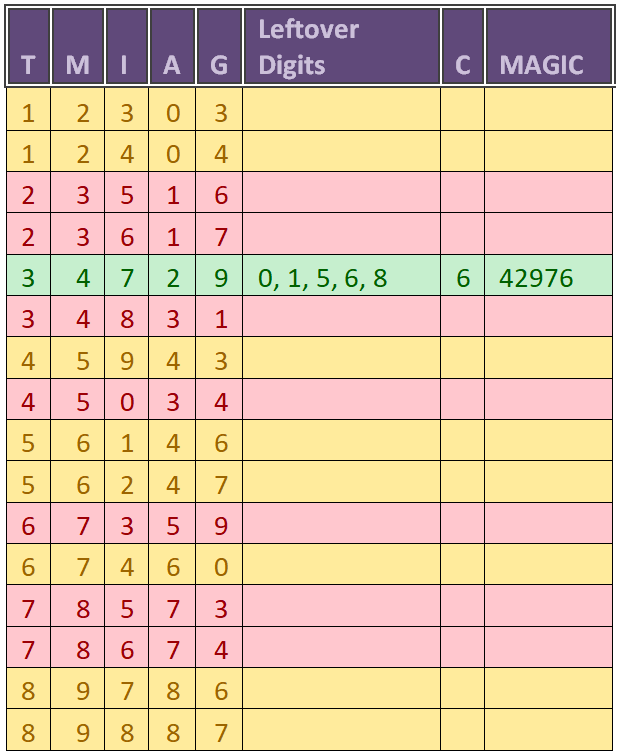
\includegraphics[scale=0.5]{guts_table}
\end{center}
Note that $A$ and $G$ are interdependent. $I+A=G$, or $I+A+1=G$ (depending on $M$ and $T$), and $J+M=A$ or $J+M+1=A$, depending on $I$ and $A$. We can find a distinct pair of $G$ for each triple of $(M, T, I)$. Everything in red does not have an even $A$, and everything in yellow does now have distinct digits. The remaining option is in green, with the only possibilities for $O$ and $H$ are 1 and 5, with $C$ being 6. Thus,  $MAGIC=\boxed{42976}$.
\end{solution}


\newpage
\section*{Set 8}
\begin{problem}
What is $\frac{1}{1\cdot2}+\frac{1}{2\cdot3} + \frac{1}{3\cdot4} + \dots + \frac{1}{29\cdot30}$?
\end{problem}

\begin{answer}
$\frac{29}{30}$
\end{answer}

\begin{solution}
Note that $\frac{1}{n(n+1)} = \frac{1}{n} - \frac{1}{n+1}$. Thus, the expression evaluates to $\frac{1}{1} - \frac{1}{2} + \frac{1}{2} - \frac{1}{3} + ... - \frac{1}{29} + \frac{1}{29} - \frac{1}{30} = 1-\frac{1}{30} = \boxed{\frac{29}{30}}$
\end{solution}


\begin{problem}
Allen, Bobby, Charles, and $49$ other people are in a math class together. The teacher randomly gives each of the $52$ students one card each from a single deck of $52$ cards (everyone receives a different card). Any student who receives either an ace, king, queen, or jack is required to do extra homework. What is the probability that at least one of Allen, Bobby, and Charles has to do extra homework? (Note: There are four aces, four kings, four queens, and four jacks in a standard deck of $52$ cards.) 
\end{problem}

\begin{answer}
$\frac{44}{65}$
\end{answer}

\begin{solution}
We will solve this by complementary counting. There are 16 total cards which would give students extra homework, so there are $36$ out of $52$ cards which do not give students extra homework. The probability that none of Allen, Bobby, and Charles have to do extra homework is therefore $\dfrac{36}{52}\cdot \dfrac{35}{51} \cdot \dfrac{34}{50} = \dfrac{21}{65}$. Thus, the probability that one of the three students gets extra homework is $1-\dfrac{21}{65} = \boxed{\dfrac{44}{65}}$.
\end{solution}


\begin{problem}
Franklyn can finish two cryptography assignments in 10 minutes, Katherine can finish one in 30 minutes, and Will Sun can finish one in 15 minutes. How long (in hours) will it take for them working together to finish six cryptography assignments?
\end{problem}

\begin{answer}
$\frac{1}{3}$
\end{answer}

\begin{solution}
It takes Franklyn 5 minutes to finish one assignment, Katherine 30, and Will 15. Thus, in 30 minutes, Franklyn finishes 6 assignments, Katherine 1, and Will 2, for a total of 9 assignments. Using proportions, we see that it takes them 20 minutes, or $\boxed{\frac{1}{3}}$ hours.
\end{solution}


\begin{problem}
A strange clock has minute and hour hands of the same length. Consider a vertical line $l$ drawn through the ``6" and ``12" numbers on the clock.
How many times a day are the hour and minute hands reflections of each other through the line $l$?
\end{problem}

\begin{answer}
26
\end{answer}

\begin{solution}
This holds at $12:00$, once between $12:00$ and $1:00$, once between $1:00$ and $2:00$, once between $3:00$ and $4:00$, and so on until once between $11:00$ and $12:00$, for a total of $13$ times in a time period of $12$ hours. Thus, our answer is $13 \times 2 = \boxed{26}$.
\end{solution}

\end{document}
